\chapter{Mathematical Model Formulation}
\label{chap:3}

This chapter serves to introduce the formal notation and state-space formulation that will be used consistently throughout this document.
\section{Variables}
\label{sec:1}
% TODO could maybe link to a paper where this formal notation is introduced.
In this section, the variables used in the model components are presented and clarified.

\begin{description}[align=left, labelwidth=3cm, leftmargin=!]
    \item[\( SoC_t \)] The amount of energy (in MWh) stored in the battery at time \( t \).
    \item[\( p_t \)] The imbalance price (€/MWh) on the electricity grid at time \( t \).
    \item[\( x_t \)] The amount of power (in MW) bought from the grid (\( x_t > 0 \)) or sold to the grid (\( x_t < 0 \)) during the interval at time \( t \).
    \item[\(A^{c}_{t}, A^d_t\)] Accumulated energy (in MWh) traded within a 15-minute quarter. They are reset to zero at the beginning of a new quarter.
    \item[\(r^{chg}, r^{dis}\)] maximum charge/discharge rate in (MW).
\end{description}

\section{Model Components}

\begin{enumerate}
    \item \textbf{State Variable ($S_t$)} \\
    The state at time $t$ consists of the current battery state of charge, the price of electricity at time t, which is a forecast if $(t + 1) \mod 15 \neq 0$ given a quarter starts at time $t \pmod{15} == 0$:

    \[
        S_t = (SoC_t, p_t, A^{c}_{t}, A^{d}_{t})
    \]
    
    \item \textbf{Decision Variable ($x_t$)} \\
    The decision variable $x_t$ represents the net energy flow to or from the battery during the time interval at time $t$. A positive value ($x_t > 0$) indicates charging, while a negative value ($x_t < 0$) indicates discharging. This decision is subject to the physical constraints of the battery system.
    
    Let $SOC_t$ be the energy stored in the battery at the beginning of the interval, $SOC^{max}$ be the maximum battery capacity, and $r^{chg}$ and $r^{dis}$ be the maximum charge and discharge rates (in energy per time interval), respectively. The decision $x_t$ must satisfy the following constraints:
    
    \begin{align*}
        x_t &\le SoC^{max} - SoC_t && \text{(Cannot charge more than available capacity)} \\
        x_t &\ge -SoC_t && \text{(Cannot discharge more than stored energy)} \\
        x_t &\le r^{chg} && \text{(Cannot charge faster than the maximum charge rate)} \\
        x_t &\ge -r^{dis} && \text{(Cannot discharge faster than the maximum discharge rate)}    
    \end{align*}

    \item \textbf{Exogenous Information ($W_{t+1}$)} \\
    This is the new, unknown information that arrives after decision $x_t$ is made.
    \[
        W_{t+1} = (p_{t+1})
    \]

    \item \textbf{Transition Function} \\
    \[
        SoC_{t+1} = SoC_t + x_t
    \]
    \[
        A^c_{t+1} = 
        \begin{cases} 
            0 & \text{if } (t+1) \pmod{15} = 0 \\
            A^c_t + \max(0, x_t) & \text{otherwise}
        \end{cases}
    \]
    \[
        A^d_{t+1} = 
        \begin{cases} 
            0 & \text{if } (t+1) \pmod{15} = 0 \\
            A^d_t + \max(0, -x_t) & \text{otherwise}
        \end{cases}
    \]
    The price $p_{t+1}$ is observed after the transition and is independent of the action $x_t$. This gives the new state vector:
    \[ 
        S_{t+1} = (SoC_{t+1}, p_{t+1}, A^c_{t+1}, A^d_{t+1}) 
    \]

    \item \textbf{Reward Function ($R(S_t, x_t)$)} \\
    This function defines the immediate financial outcome of an action taken at time $t$. Due to market rules, financial settlement occurs only at the end of each 15-minute interval. To ensure the agent learns to balance financial gains with the physical wear of the battery, the reward function calculates the \textit{Net Profit}: the gross revenue from energy arbitrage minus the marginal degradation cost.
    
     Let $E^{net}_t = A^c_{t} - A^d_{t} + x_t$ denote the net energy traded, and $E^{thru}_t = A^c_{t} + A^d_{t} + |x_t|$ denote the total energy throughput over the quarter. Let $c_{wear}$ be the marginal degradation cost (€/MWh). The reward is defined as:
    \[
    R(S_t, x_t) = 
    \begin{cases} 
        -p_t \cdot E^{net}_t - c_{wear} \cdot E^{thru}_t & \text{if } (t+1) \pmod{15} = 0 \\
        0 & \text{otherwise}
    \end{cases}
    \]
    $-p_t \cdot E^{net}_t$ represents the gross financial settlement, and  $c_{wear} \cdot E^{thru}_t$ represents the physical wear-and-tear cost of the energy throughput.  \\
    A positive $R$ indicates a net profit, and a negative $R$ indicates a net loss.
    
    \item \textbf{Objective Function} \\
    The goal of the agent is to find an optimal policy $\pi^*$ that maximizes the expected cumulative discounted reward over an episode of length $T$. Formally, the objective function $J(\pi)$ is defined as:
    \[
        \max_{\pi} J(\pi) = \max_{\pi} \mathop{\mathbb{E}} \left[ \sum_{t=0}^{T} \gamma^t R(S_t, x_t) \right]
    \]
    where:
    \begin{itemize}
        \item $\mathop{\mathbb{E}}$ denotes the expected value given the stochastic nature of the environment (prices).
        \item $\gamma \in [0, 1]$ is the discount factor, determining the importance of future rewards.
    \end{itemize}
\end{enumerate}

\section{Battery Degradation Modeling}
To accurately evaluate the profitability of an energy arbitrage agent, the physical wear of the battery system must be financially quantified. Without penalizing energy throughput, an agent would naturally execute ``micro-cycles''---charging and discharging continuously for negligible price spreads---which rapidly destroys the battery's lifespan while generating minimal revenue.

To counteract this, a constant marginal degradation cost, denoted as $c_{wear}$ (€/MWh), is introduced into the reward function. This cost is derived using a straightforward linear depreciation model based on the total capital investment and the expected lifetime throughput of the battery:
\[
    c_{wear} = \frac{\text{Total Capital Cost}}{\text{Capacity} \times \text{Maximum Cycles} \times 2}
\]
where the denominator calculates the total lifetime energy throughput (multiplying by two because one full cycle consists of both charging and discharging the full capacity). For example, a 2 MWh battery system with a total capital cost of €500,000 and an expected lifespan of 80,000 cycles results in a marginal throughput cost of approximately €1.56 per MWh.

\subsubsection*{Assumptions and Limitations}
It is important to acknowledge that representing battery degradation as a constant, linear cost is a significant simplification of physical reality. In practice, lithium-ion battery degradation is a highly complex, non-linear process influenced by several dynamic operational factors:
\begin{itemize}
    TODO Confirm this with literature
    https://www.scribd.com/document/906050666/Zhou-2011

    \item \textbf{Depth of Discharge (DoD):} Deep cycles degrade the battery exponentially faster than shallow micro-cycles.
    \item \textbf{State of Charge (SoC):} Resting at extreme states (e.g., near 0\% or 100\% charge) accelerates capacity fade.
    \item \textbf{C-rate:} Charging or discharging at maximum power generates more heat and stress than operating at lower power levels.
\end{itemize}

Furthermore, the maximum cycle counts provided by battery manufacturers are typically determined under highly optimistic, tightly controlled laboratory conditions. These ideal benchmarks rarely reflect the harsh, variable stress induced by aggressive real-world market trading. 

While incorporating an advanced, non-linear electrochemical degradation model would provide a more accurate assessment of the true trading costs, it would drastically increase the complexity of the state space and the reward landscape. Therefore, for the scope of this thesis, degradation is approximated as a linear, static cost. Integrating sophisticated battery health modeling directly into the reinforcement learning environment remains a highly relevant for future research.

\section{State Space Decisions}
In this section some extra context is given to the decisions of adding certain features.
\subsection{\(A^c_t, A^d_t\): Tracking Intra-Quarter Trading}
    The original state representation, $S_t = (SoC_t, p_t)$, was found to be insufficient for the agent to properly assign credit for its actions within a 15-minute settlement period. This created a critical ambiguity, which can be illustrated by comparing two scenarios:
    
    \begin{itemize}
        \item \textbf{Case 1:} The agent starts a 15-minute period with a full battery. It remains idle for 14 minutes and then discharges in the final minute. The reward for this quarter is positive, calculated as $R \approx x_{discharge} \cdot p_{15}$.
        
        \item \textbf{Case 2:} The agent starts the period with an empty battery. It charges the battery full in the first minute, holds the charge, and then discharges in the final minute. The reward for this quarter is significantly lower (likely negative), as it is based on the net energy traded: $R \approx (-C_{capacity} + x_{discharge}) \cdot p_{15}$.
    \end{itemize}
    
    In both cases, the state of the battery ($SoC_{14}$) and the action taken ($x_{14}$) in the final minute are identical. However, the agent receives a vastly different reward. This complicates the learning process, as the agent cannot distinguish between these two histories based solely on the current state.
    
    To resolve this ambiguity, the state space was augmented with two new features:
    \begin{itemize}
        \item \(A^c_t\): The total energy charged within the current quarter up to time $t$.
        \item \(A^d_t\): The total energy discharged within the current quarter up to time $t$.
    \end{itemize}

    \paragraph{Justification for Two Separate Features}
    A natural question is why two separate features are used instead of a single feature representing the net energy traded, e.g., $A^{net}_t = A^c_t - A^d_t$. While this would solve the primary ambiguity described above, it would introduce a new one. Consider two distinct scenarios:
    
    \begin{itemize}
        \item \textbf{Scenario A:} The agent charges for 7 minutes and then discharges for 7 minutes. The net energy traded is close to zero ($A^{net}_t \approx 0$), but the total charged and discharged volumes are significant ($A^c_t > 0, A^d_t > 0$).
        
        \item \textbf{Scenario B:} The agent remains idle for 14 minutes. The net energy traded is zero ($A^{net}_t = 0$), and the charged and discharged volumes are also zero ($A^c_t = 0, A^d_t = 0$).
    \end{itemize}
    
    With a single net feature, these two scenarios would be indistinguishable to the agent. However, Scenario A involves significant energy cycling, which is far more costly from a battery degradation perspective. By keeping $A^c_t$ and $A^d_t$ separate, the state representation preserves this crucial information about total energy throughput. This allows the agent to correctly correlate its actions to the final reward and provides a foundation for potentially modeling costs like battery degradation in the future.

\section{Data and Preprocessing}
% TODO check if there is some paragraph about the i.i.d assumption, why it is hard here, and where should we account for it.
This section details the data acquisition, preprocessing steps, exploratory analysis, and the partitioning strategy utilized for training and evaluating the reinforcement learning agents. 

\subsection{Data Provenance and Characteristics}
The primary data source for this research is Elia, the Belgian Transmission System Operator (TSO). The dataset provides electricity imbalance market data at a 1-minute resolution, accessible via Elia's OpenData platform. 

A critical characteristic of this dataset is the distinction between forecasts and settlement prices. For every minute $t$, the published price is an indicative forecast. The definitive financial settlement price is only established at the end of each 15-minute quarter (i.e., when $t \pmod{15} = 0$). This 1-minute forecast data has only been available since the implementation of the MARI (Manually Activated Reserves Initiative) platform on May 21, 2024. Consequently, the primary dataset utilized in this research is restricted to data generated after this date.

\subsubsection{Legacy Data Integration}
While the core focus remains on post-MARI data, incorporating historical (pre-MARI) data can be theoretically valuable for expanding the training set. However, doing so requires preprocessing and harmonization. The primary challenge lies in the evolution of the pricing model. The legacy format utilizes distinct columns for positive and negative imbalance prices, whereas the current format provides a single, unified imbalance price. 

To integrate these datasets, legacy data must be collapsed into a single column by selecting the price corresponding to the system imbalance direction at each timestamp. Furthermore, technical naming shifts—such as the transition from "Net regulation volume" to "Area Control Error" (ACE)—require explicit feature mapping to maintain continuity in volume metrics. Finally, the feature space must be aligned by either pruning deprecated indicators (e.g., the strategic reserve price) or applying consistent padding to new analytical features (e.g., Alpha) to ensure uniform dimensionality across the entire simulation horizon.


\subsection{Data Partitioning Principles}
While analytical methods exist to solve Markov Decision Processes (MDPs) when transition probabilities are perfectly known, the complex and unpredictable nature of electricity imbalance prices renders exact mathematical solutions intractable in practice. To overcome this, this research utilizes Reinforcement Learning (RL). RL is particularly advantageous for energy arbitrage because it is a ``model-free'' approach; it can optimize policies in stochastic, continuous, and highly volatile environments by learning directly from interactions with historical data, entirely bypassing the need for an explicit mathematical model of the market's underlying dynamics \cite{VAZQUEZCANTELI20191072}. 

To evaluate an RL agent's true generalization capabilities in unseen market conditions, it is fundamental to evaluate it on distinct and statistically separated datasets. In standard machine learning, the validity of such an evaluation relies heavily on the assumption that data points are Independent and Identically Distributed (i.i.d.) \cite{pmlr-v119-hsieh20a}. However, continuous time-series data from energy markets inherently violates both components of the i.i.d. assumption. Consequently, the specific methodology used to partition this data requires careful deliberation; a rigorously designed splitting strategy is essential to overcome these statistical violations and ensure that the evaluation metrics provide an as unbiased estimate of the agent's real-world performance as possible.

When partitioning time-series data, these i.i.d. violations manifest as two primary risks that must be balanced:
\begin{enumerate}
    \item \textbf{Loss of Representativeness (Violating Identical Distribution):} A strict chronological split (e.g., reserving the final 20\% of the timeline for testing) often isolates the evaluation to a specific season. Given the non-stationary nature of energy prices, a model might overfit to the test period's specific regime (e.g., winter) and fail to generalize to others. While this bias diminishes with very large, multi-year datasets where the test set encompasses several full seasonal cycles, the relatively short duration of the available post-MARI dataset (less than two years) renders chronological splitting highly unrepresentative, as the training and testing sets fail to share identical statistical distributions.
    
    \item \textbf{Data Leakage (Violating Independence):} If data is simply shuffled randomly, the temporal sequence is broken, preventing the model from learning sequential patterns. Furthermore, because latent variables cause adjacent data points to be highly autocorrelated, the data points are not statistically independent. Placing day $X$ in the training set and day $X+1$ in the test set exploits this lack of independence, causing information leakage that results in artificially inflated evaluation scores.
\end{enumerate}

To successfully navigate these risks and design an appropriate partitioning strategy, it is first necessary to conduct an exploratory data analysis. Understanding the underlying structural characteristics of the imbalance prices—such as seasonality, stationarity, and autocorrelation—dictates exactly how the data must be handled to correct these i.i.d. violations and prevent biased evaluation.

\subsection{Exploratory Data Analysis}
% TODO, dit kwam na het gesprek met prof Dambre, bespreek ook een keer wanneer out of sample wel een goeie keuze is, er kwam ter sprake dat de data er te klein voor was om geen bias te krijgen op seasonality.

\begin{figure}[h]
	\centering
	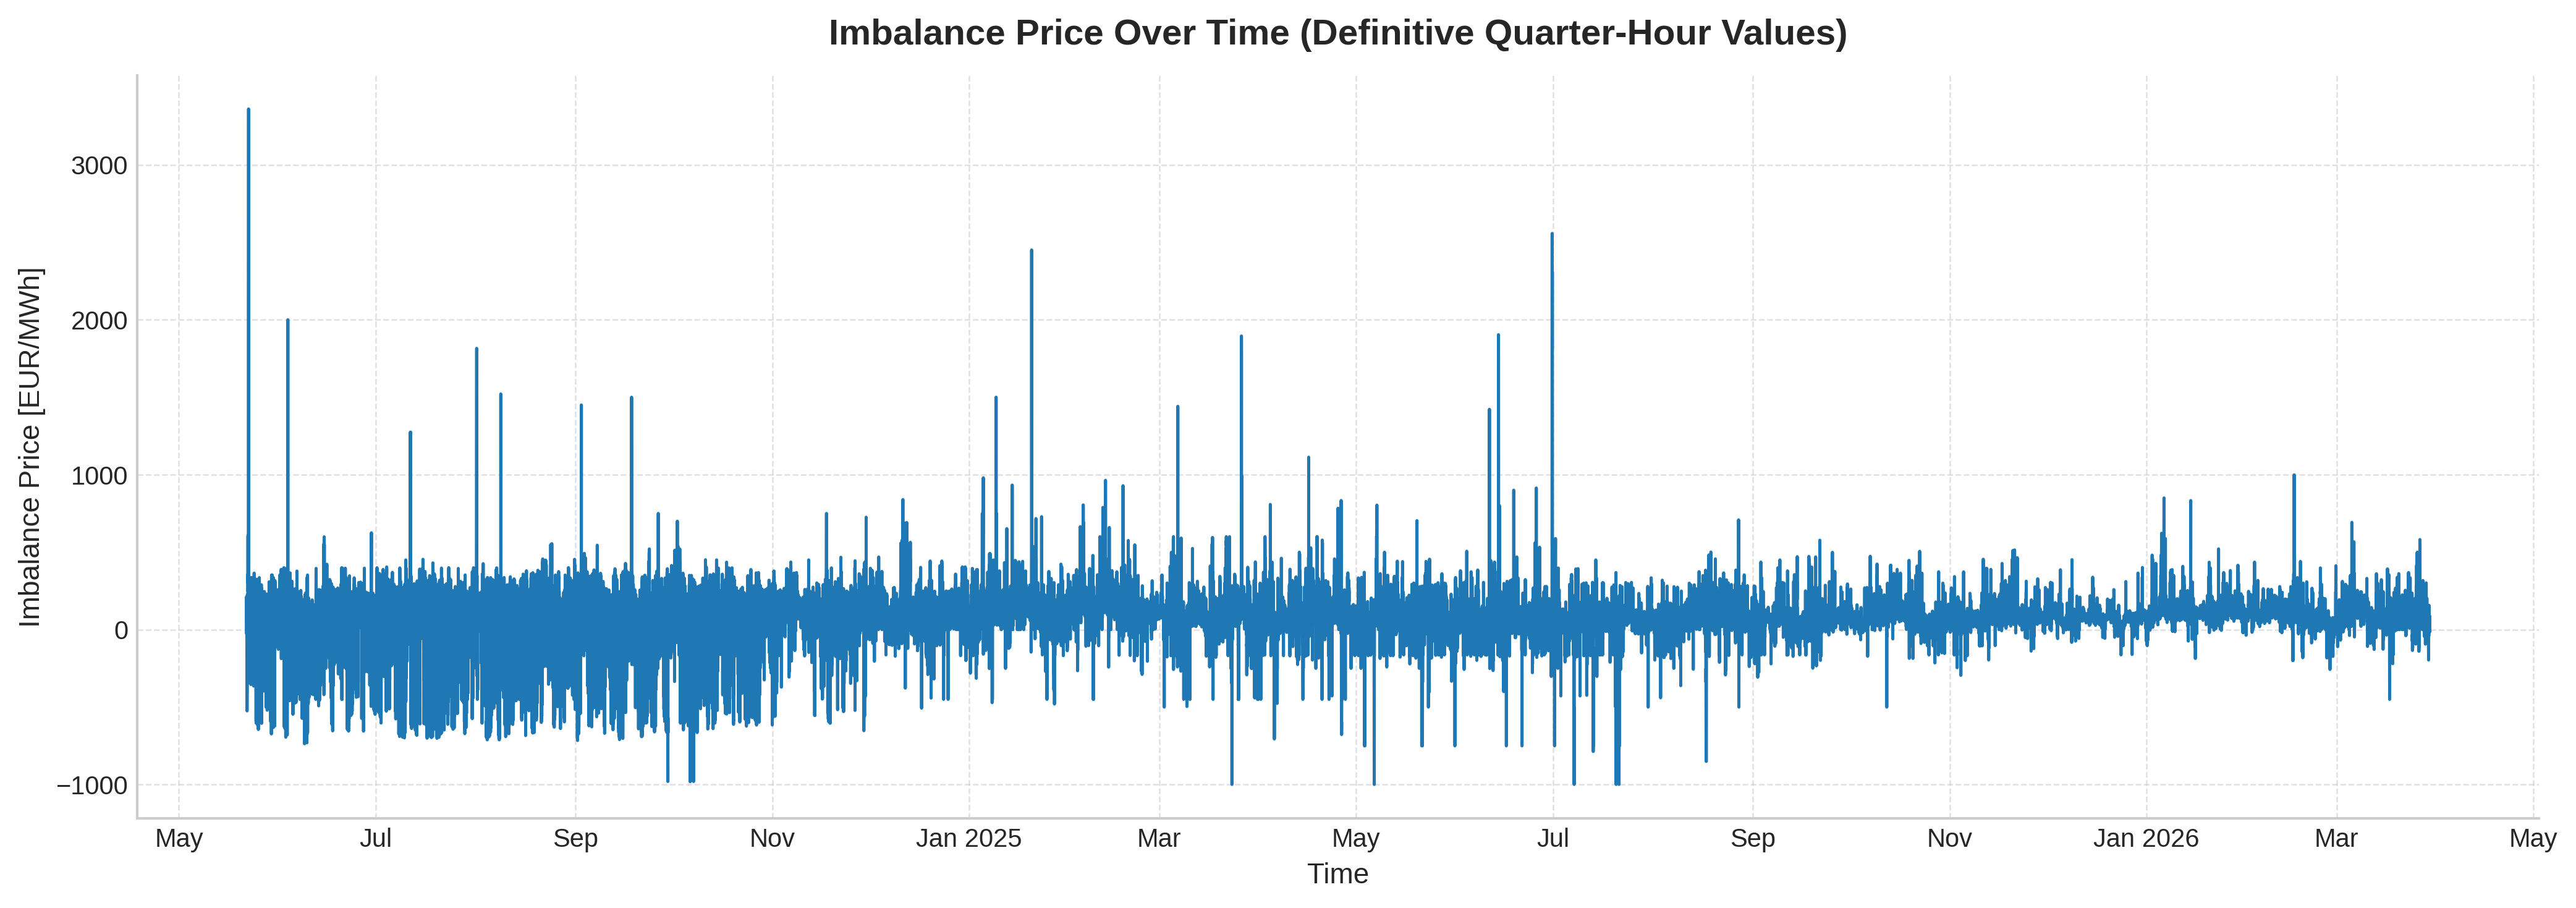
\includegraphics[width=\textwidth]{images/data/imbalance_price_thesis.png}
	\caption{Evolution of the final quarter imbalance prices across the entire dataset.}
	\label{fig:imb_price_full}
\end{figure}

Figure \ref{fig:imb_price_full} provides a macro-level overview of the imbalance prices across the available timeline. Before proceeding to an in-depth analysis, a visual inspection of the timeline can help us identify prominent characteristics.

Most notably, the variance of the imbalance prices decreases significantly after November 2024. This drop in volatility coincides with Elia's integration into the PICASSO platform (Platform for the International Coordination of Automated Frequency Restoration and Stable System Operation). By enabling the continuous cross-border exchange of balancing energy, PICASSO increased market liquidity and significantly dampened extreme, localized price spikes within the Belgian grid.

This distinct regime shift naturally raises the question of whether the highly volatile, pre-PICASSO data remains suitable for training a model expected to operate in current, more stable market conditions. However, retaining this historical data provides valuable extra context. Exposing the model to more extreme price events expands its experiential state space, forcing it to learn risk-management and deep arbitrage (leverage) strategies.

Furthermore, the timeline shows frequent high price spikes during the summer months. In contrast, the winters of 2024-2025 and 2025-2026 remain much more stable, with almost no extreme spikes. This points to a much higher variability in the summer, which is a key characteristic we will need to investigate further.

\subsubsection{Seasonality and Stationarity}
\label{Seasonality_and_stationarity}
Initial analysis indicates that the imbalance market is highly non-stationary over short horizons. The statistical properties of the prices (mean, variance) change significantly depending on the season and time of day. 

\begin{figure}[h]
    \centering
    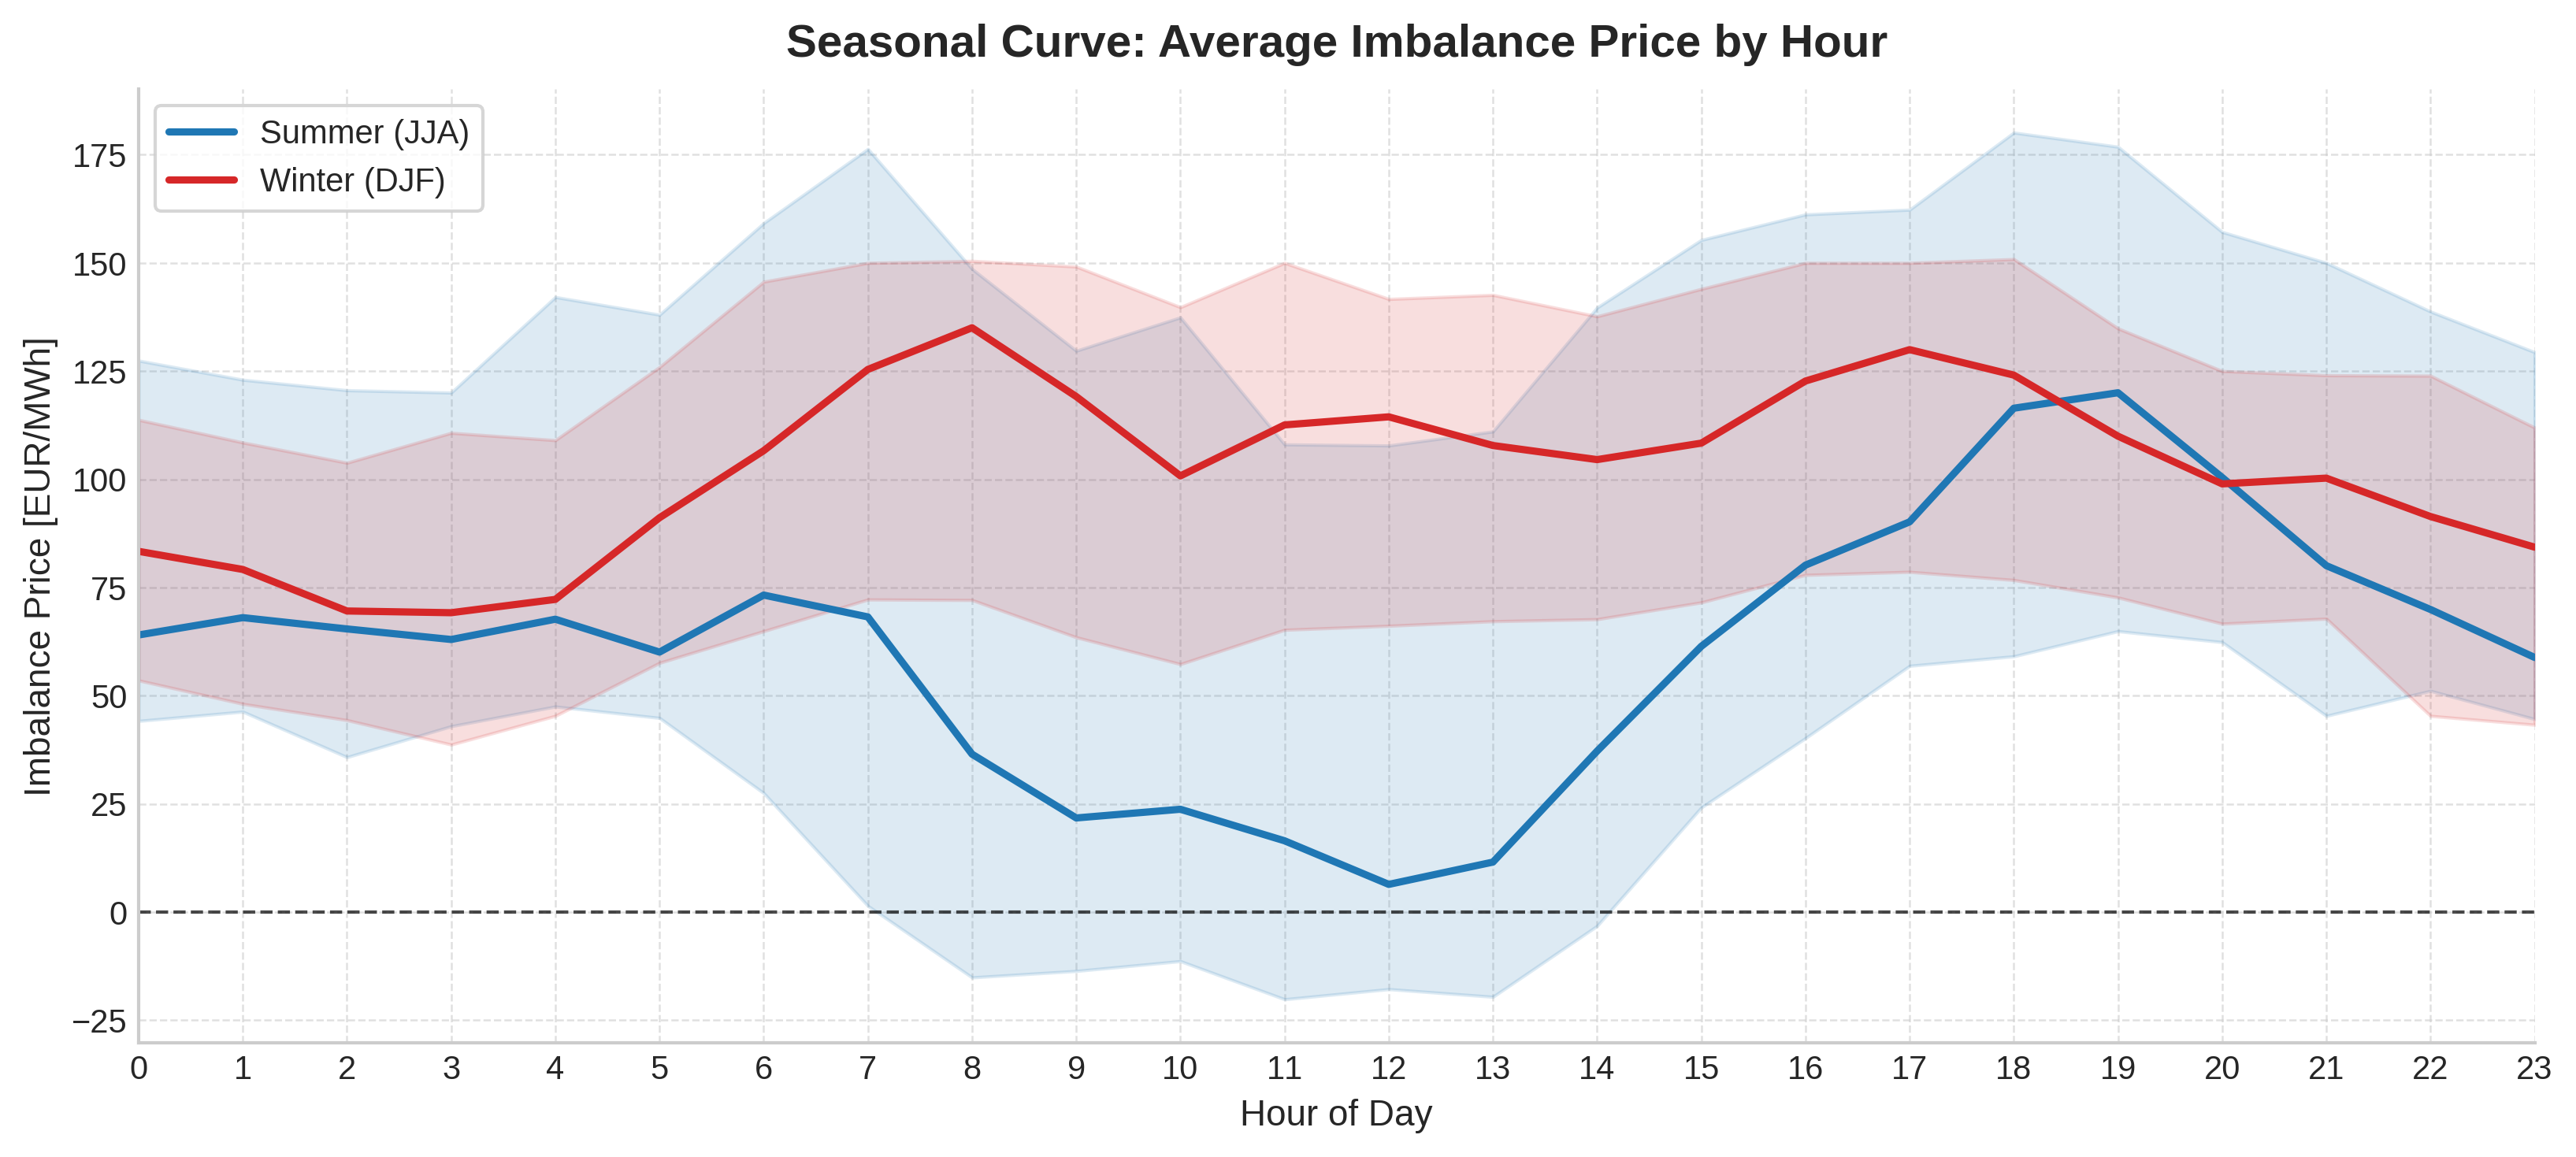
\includegraphics[width=\textwidth]{images/data/curve_summer_winter_prices.png}
    \caption{Average imbalance price profile during summer and winter months. Shaded regions represent standard deviation.}
    \label{fig:seasonal_curve}
\end{figure}

Figure \ref{fig:seasonal_curve} depicts the average hourly imbalance price profiles for both summer (June, July, August) and winter (December, January, February) seasons. The plot reveals two key characteristics of the electricity market:
\begin{enumerate}
    \item \textbf{Intraday Predictability:} There exists a clear and consistent daily rhythm. Prices tend to peak in the early evening (18:00-20:00) and reach a minimum during the pre-dawn hours (03:00-05:00). This predictability enables the model to leverage anticipated intraday demand fluctuations.
    \item \textbf{Inter-Seasonal Regime Shifts:} The shape of the hourly price profile is fundamentally different depending on the season. In winter, the intraday peak is more pronounced and occurs at a higher average price, whereas the summer profile is characterized by a midday dip. Furthermore, as indicated by the wider shaded regions in Figure \ref{fig:seasonal_curve}, the standard deviation is significantly higher during the summer months compared to the winter. This increased variance reflects a higher degree of price uncertainty and volatility, likely driven by the weather-dependent nature of solar photovoltaic generation during the day.
\end{enumerate}

These observations define the two fundamental requirements for the data partitioning strategy: it must preserve local temporal dependencies while simultaneously ensuring global seasonal representativeness.

First, to preserve local temporal dependencies, the strategy must avoid the random shuffling of individual data points. Time-series data inherently exhibits \textit{autocorrelation}—the strong statistical similarity between a given time step and its immediate predecessors. In the context of electricity markets, the price at minute $t$ is highly dependent on the price at $t-1$. If individual minutes are randomly assigned to different datasets, this dependency is exploited. It leads to severe data leakage, allowing the model to artificially "predict" test set values simply by recalling adjacent minutes from the training set. To prevent this, the data must be partitioned into contiguous blocks (or \textit{episodes}). Maintaining continuous time blocks not only prevents leakage but also preserves the sequential logic required for arbitrage (e.g., the transition from a low-price charging period to a high-price discharging peak).

Second, to ensure global seasonal representativeness, these contiguous blocks cannot be drawn from just one segment of the timeline. Due to the significant regime shifts and varying volatility levels observed between summer and winter, the evaluation samples must be drawn from across the entire annual cycle. Testing the model against a diverse, year-round mixture of market conditions prevents the evaluation from being biased toward a single seasonal profile. 

By combining these two principles—sampling intact, multi-day episodes from across the entire calendar year—the partitioning strategy provides a robust and mathematically sound foundation for evaluating the agent's true generalization capabilities.

An analysis of the year-long dataset, visualized in Figure \ref{fig:monthly_correlation_boxplot_curve}, provides further insight into the nature of this time-series.

\begin{figure}[h]
\centering
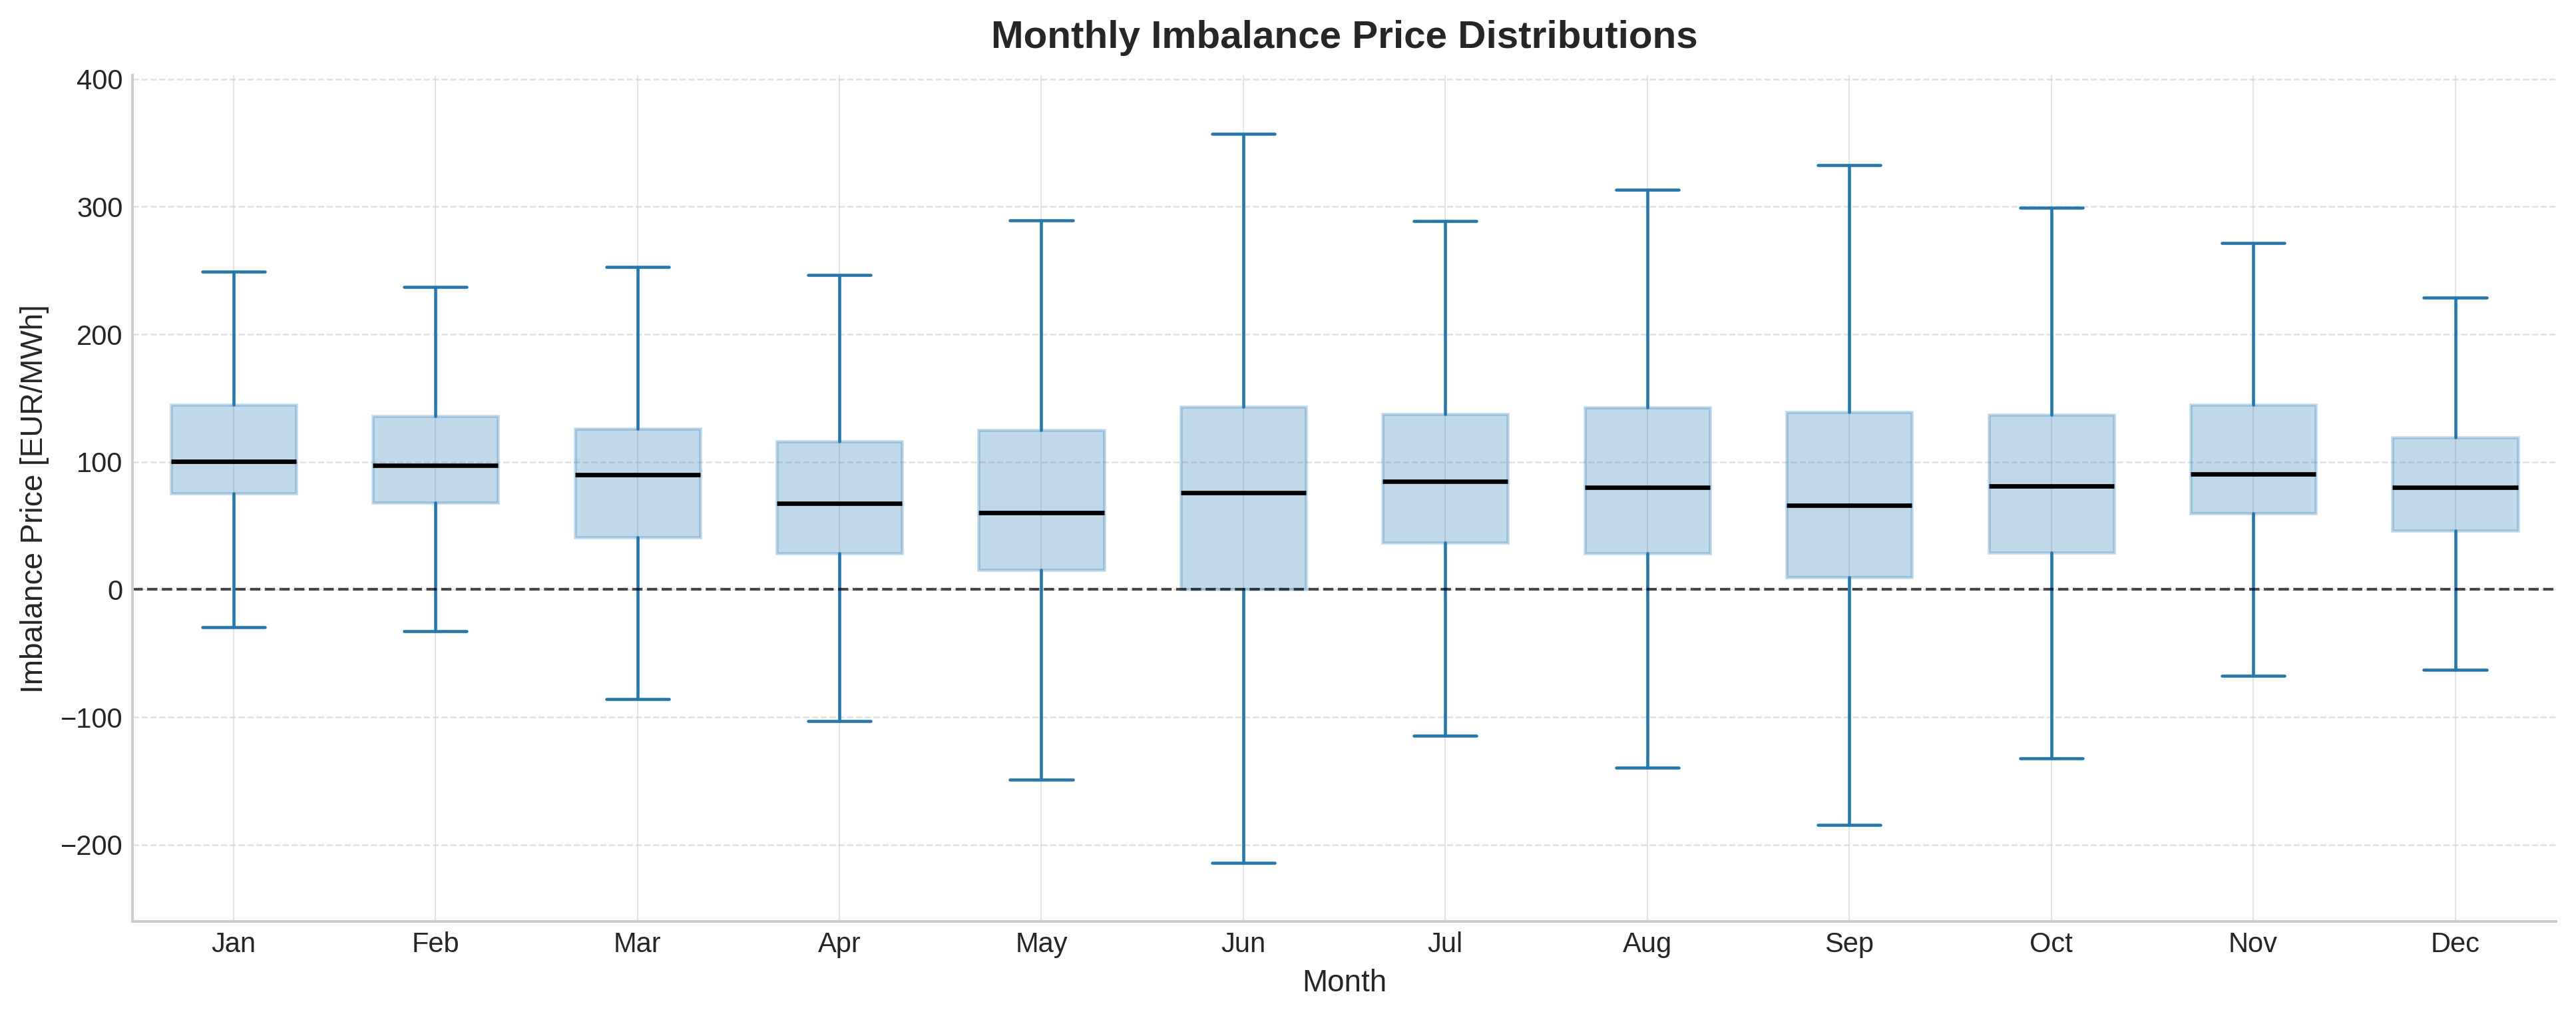
\includegraphics[width=\textwidth]{images/data/monthly_price_distributions_boxplot.png}
\caption{Monthly Distribution of Belgian Imbalance Prices illustrating seasonal volatility shifts.}
\label{fig:monthly_correlation_boxplot_curve}
\end{figure}

The boxplot distributions demonstrate that while the global mean of the imbalance price remains relatively stable across the months, the variance (volatility) fluctuates significantly throughout the year. This stability in the mean suggests that the data exhibits a degree of weak-form stationarity. Because the fundamental price baseline does not drift into a non-stationary "random walk" (as is often the case with stock prices), partitioning the data into separate training, validation, and testing sets remains a mathematically valid approach. Provided that the sampling blocks are large enough to capture local autocorrelation, the model will encounter statistically similar price distributions in both the training and evaluation phases, allowing for a reliable assessment of its generalization capabilities.

\begin{figure}[h]
\centering
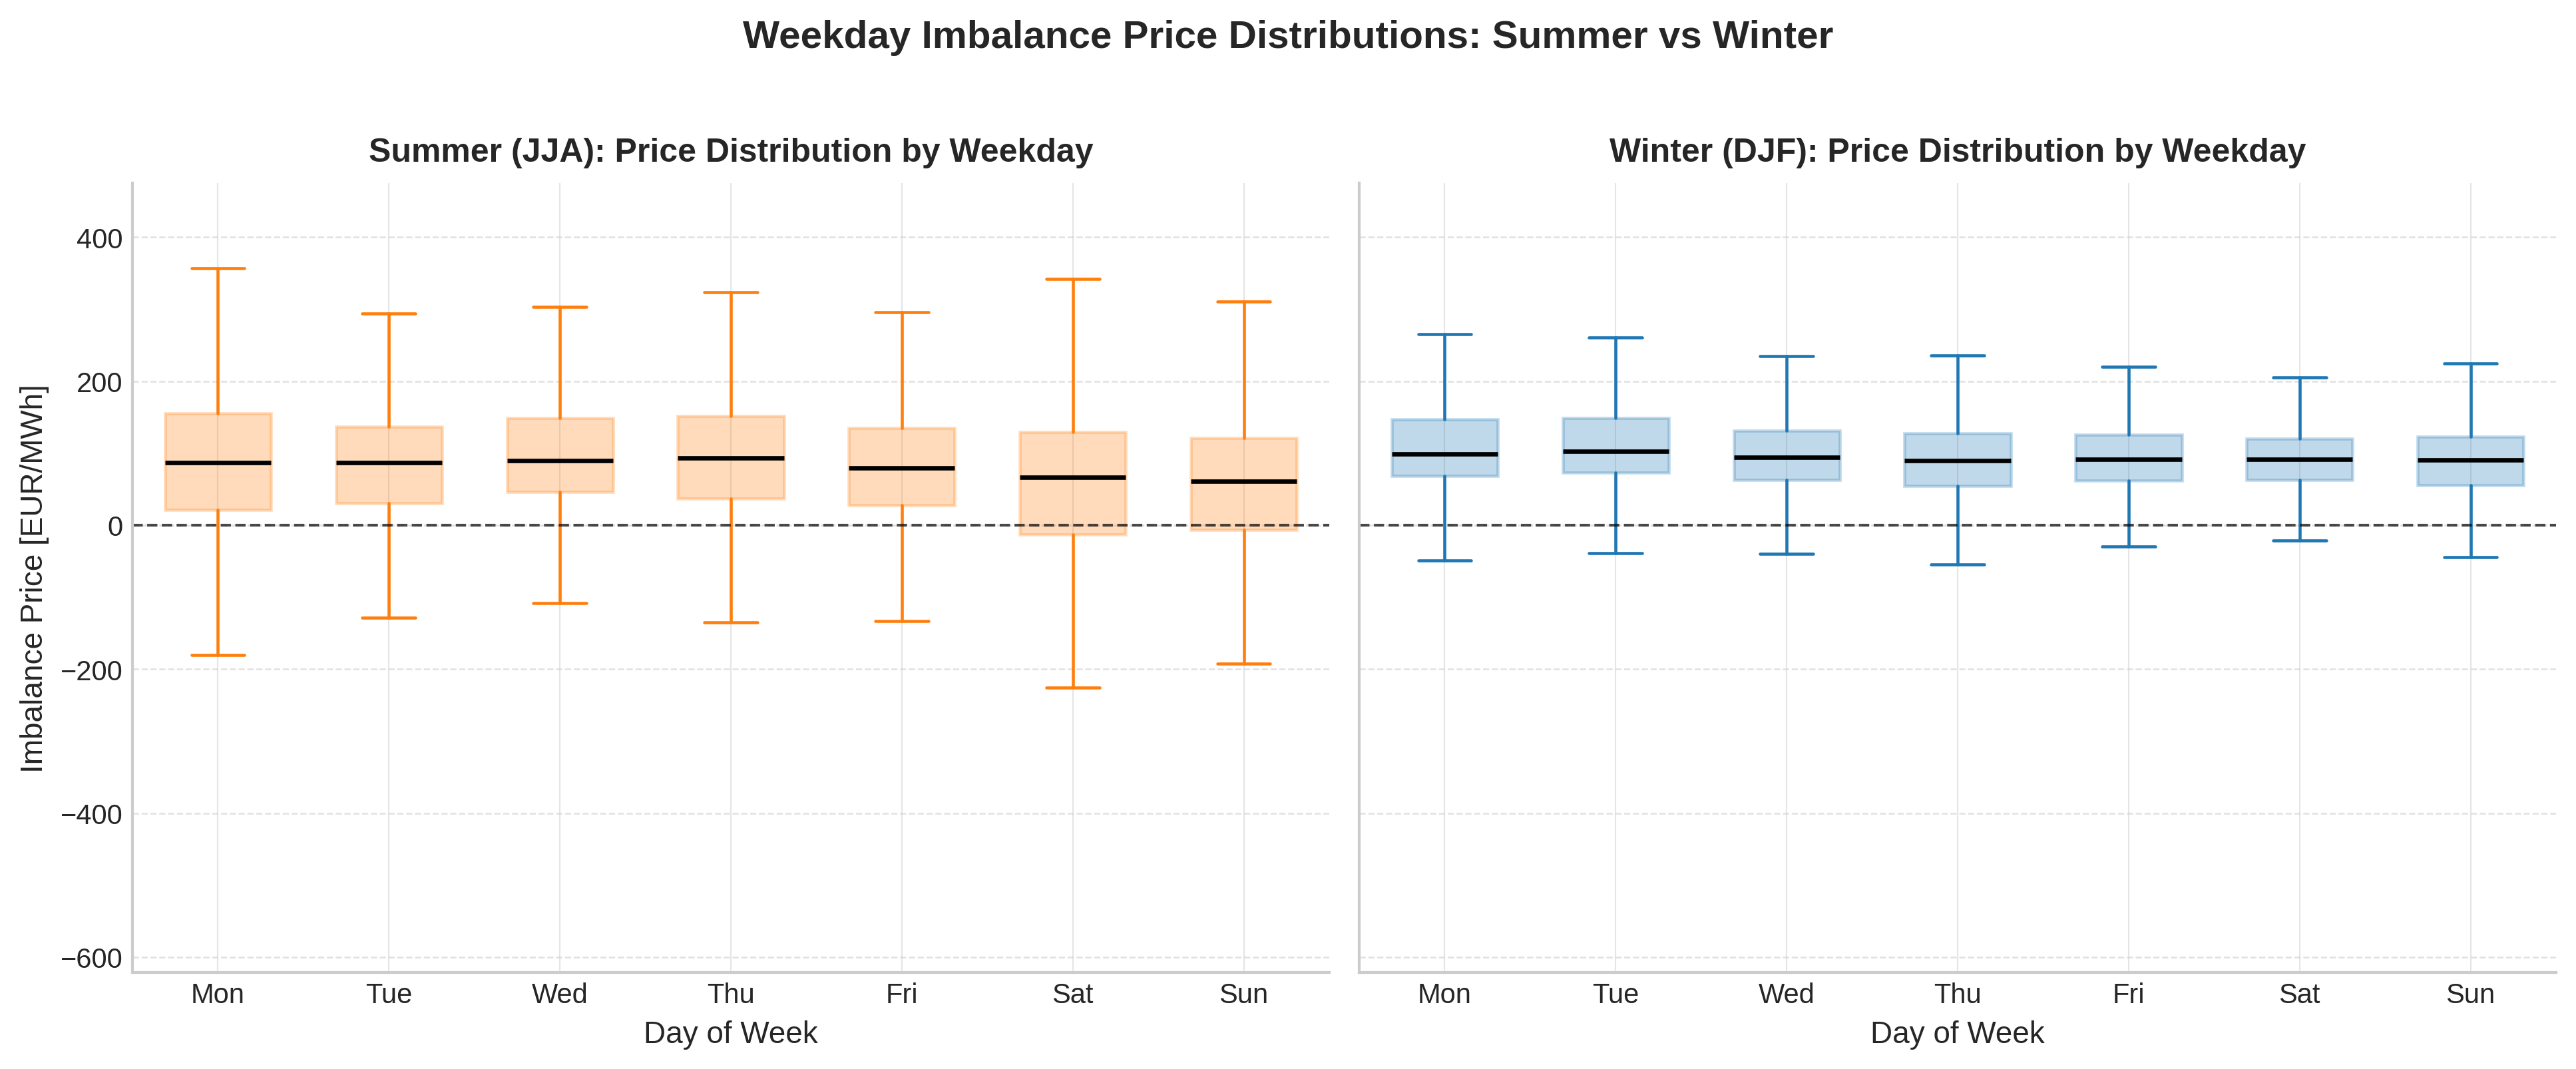
\includegraphics[width=\textwidth]{images/data/weekday_boxplots_summer_vs_winter.png}
\caption{Weekly Distribution of Belgian Imbalance Prices illustrating weekly and seasonal volatility shifts.}
\label{fig:weekly_correlation_boxplot_curve}
\end{figure}

Figure \ref{fig:weekly_correlation_boxplot_curve} reaffirms the contrast between winter and summer regimes, displaying a consistent mean but a distinct difference in variance. Furthermore, it demonstrates that weekly correlation is almost non-existent. Consequently, the contiguous sampling blocks do not need to span across multiple weeks to capture day-to-day dependencies, as such long-term weekly correlations barely exist in this specific market.

\subsection{Data Partitioning: $K$-fold $hv$-Block Cross-Validation}
In traditional time-series forecasting, models are typically evaluated using an out-of-sample (OOS) or ``last block'' validation approach, where the final chronological portion of the data is reserved for testing. However, extensive empirical studies by Bergmeir and Benítez \cite{BERGMEIR2012192} demonstrate that last-block evaluation fails to make full use of the available information and yields significantly less robust error estimates compared to cross-validation techniques. To leverage the statistical robustness of cross-validation while circumventing the theoretical violations of the independent and identically distributed (i.i.d.) assumption caused by temporal autocorrelation, they propose blocked evaluation methodologies as the superior standard procedure \cite{BERGMEIR201870}.

Building on this theoretical foundation, this research abandons the single train-test holdout approach in favor of \textbf{$K$-fold $hv$-block cross-validation}. These two concepts work in tandem: standard $K$-fold cross-validation provides the overarching framework for robustness by training $K$ distinct models and comparing their performance across $K$ independent validation and test sets \cite{BROWNE2000108}. However, to safely construct these $K$ uncorrelated sets from continuous time-series data without causing leakage, the $hv$-blocking technique is utilized. This methodology systematically rotates the training and evaluation sets across the folds, maximizing data utilization \cite{RACINE200039}. The components of this approach map to established statistical theory as follows:

\begin{itemize}
    \item \textbf{Blocked Partitioning (The $v$-block):} Instead of partitioning the data by individual randomized timestamps (which destroys sequence dependencies), the continuous dataset is divided into discrete, contiguous blocks of length $v$ (e.g., multi-day episodes). As demonstrated in the exploratory data analysis \ref{Seasonality_and_stationarity}, the electricity imbalance price time-series satisfies the condition of stationarity. This is a critical finding, as Bergmeir et al. \cite{BERGMEIR2012192} mathematically proved that blocked cross-validation yields robust, unbiased error estimates specifically under the assumption of data stationarity. With this theoretical prerequisite fulfilled, the $v$-blocks can be safely utilized. Furthermore, rather than keeping these blocks in strict chronological folds, they are systematically interleaved across $K$ cross-validation folds. Distributing the $v$-blocks evenly across the calendar year actively ensures that every single evaluation fold contains a representative, stratified mixture of all seasonal market regimes (e.g., both high-volatility winter weeks and low-volatility summer weekends).
    
    \item \textbf{Data Purging (The $h$-buffer):} To explicitly prevent look-ahead bias and the leakage of autocorrelated errors, temporal gaps are introduced during every iteration of the cross-validation process. This is an application of \textit{non-dependent} or \textit{$h$-block} methodology \cite{BERGMEIR2012192}. Specifically, for any given evaluation block, a gap of size $h$ (measured in hours) immediately preceding and following the block is ``purged'' (explicitly removed) from the corresponding training set. By dynamically removing this adjacent, highly correlated data at each step of the cross-validation, the evaluation sets remain rigorously isolated.
\end{itemize}

By executing the Deep Reinforcement Learning training process from scratch across all $K$ independent folds, the resulting performance metrics can be reported with a robust variance estimate, definitively proving the stability and generalizability of the learned policies across the entire dataset.

\paragraph{Dataset Roles per Fold}
During each iteration $k$ of the cross-validation process, the overarching dataset is dynamically partitioned into the following distinct roles:
\begin{itemize}
    \item \textbf{Test Set:} A predefined fraction of the $v$-blocks assigned to fold $k$. This set is strictly held out and used exclusively for final performance reporting for this specific iteration.
    \item \textbf{Validation Set:} A second fraction of the $v$-blocks assigned to fold $k$. This set is used for hyperparameter tuning and early stopping during the training phase, ensuring configuration decisions do not bias the test results.
    \item \textbf{Buffer Zones:} The $h$-hour safety margins surrounding both the Test and Validation blocks. Data within these buffers is permanently excluded from all sets in the current fold.
    \item \textbf{Training Set:} All remaining continuous chunks of data (shards) that are not claimed by the Test, Validation, or Buffer assignments.
\end{itemize}

\paragraph{Data Utilization and the Cost of Leakage Prevention}
It must be acknowledged that this approach to leakage prevention comes at a cost to data efficiency within any single training iteration. Every time a validation or test block is designated, the surrounding $h$-buffer hours are explicitly purged from that specific training set. 

However, the overarching $K$-fold cross-validation framework fundamentally mitigates this limitation. In a traditional Out-Of-Sample (OOS) chronological split, the final portion of the timeline is permanently excluded from the training phase, resulting in a permanent loss of training information. In contrast, the rotational nature of $K$-fold cross-validation ensures that every block of data is utilized for both training and evaluation across the different iterations. Data that is purged or held out in iteration $k$ seamlessly transitions into the training set during subsequent folds. This mechanism maximizes the extraction of information from the entire dataset over the course of the evaluation process, achieving high data utilization without compromising the strict temporal isolation required for an unbiased performance metric.
\subsection{Fold Characteristics and Parameter Selection}
\label{fold-characteristics}
\begin{figure}[h]
    \centering
    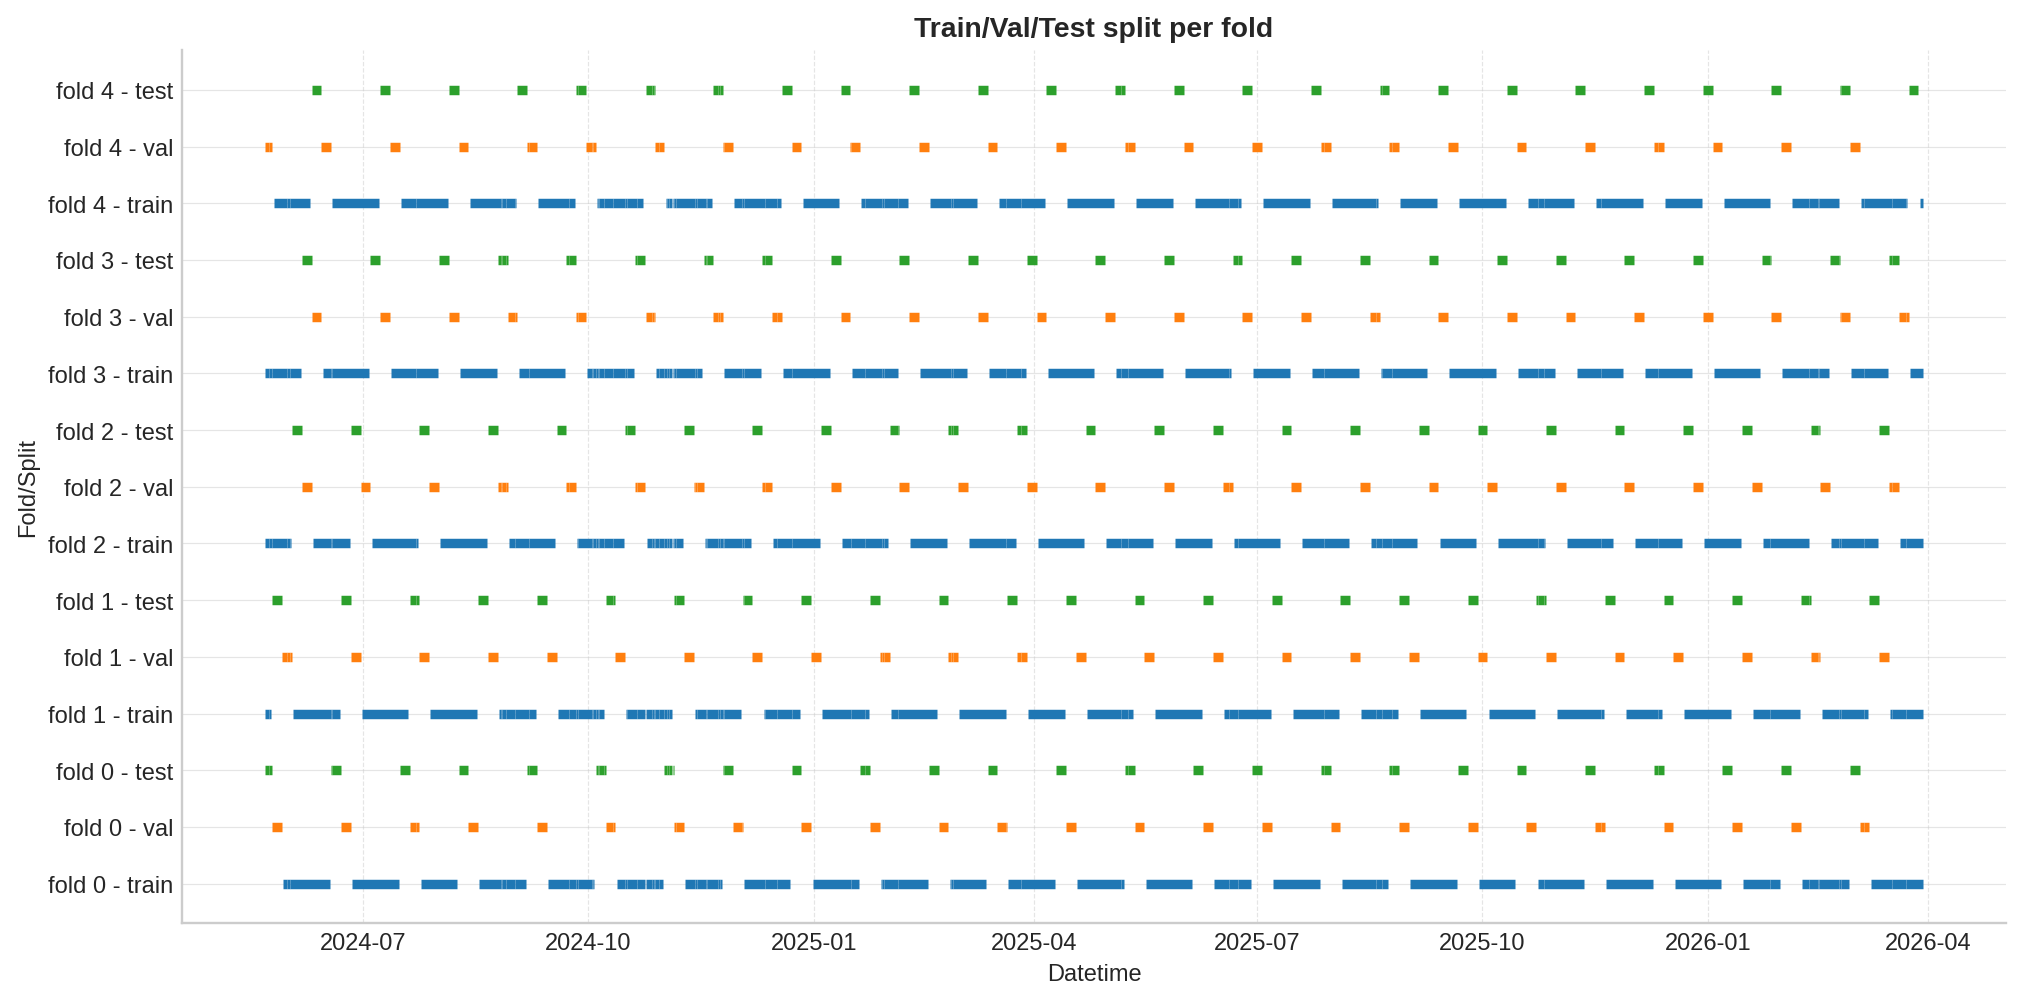
\includegraphics[width=\textwidth]{images/data/data_split_per_fold.png}
    \caption{Visualization of the data partition per fold, illustrating the contiguous training blocks and the isolated, non-overlapping validation and test episodes.}
    \label{fig:split_per_fold}
\end{figure}

This research employs a $5$-fold $4-12$-block cross-validation strategy. The choice of $K=5$ folds aligns with standard machine learning practices, providing a sufficient number of iterations to measure the generalization capabilities of the model without having a to high computational burden. 

The block size ($v$) is set to 4 days, which establishes the length of a single evaluation episode. The temporal exclusion buffer ($h$) is set to 12 hours. This buffer size represents a necessary trade-off between maximizing data utilization and ensuring security against data leakage. Given that the total dataset spans a relatively short horizon (less than two years), the 12-hour buffer was deemed sufficient to allow temporal autocorrelations to decay while preserving as much training data as possible.

The resulting data split is visualized in Figure \ref{fig:split_per_fold}. The allocation algorithm strictly guarantees that there is zero overlap between the validation and test sets across the folds. Furthermore, the evaluation periods are strategically grouped to ensure that the intervening training periods remain as continuous as possible. Highly continuous training blocks are highly desirable in Reinforcement Learning, as artificial boundaries and frequent environment resets disrupt the agent's ability to learn longer-term sequential dependencies.

To validate the efficacy of this buffered episodic splitting strategy, it is necessary to confirm that the resulting data partitions are statistically representative of one another. The sets must be independently sampled to minimize leakage, while remaining identically distributed to ensure the agent is evaluated on the same market dynamics it was trained on. %TODO cite paper that describes importance of i.i.d and its relevance to leakage and features.

\subsubsection{Feature Distribution Homogeneity}
A core assumption of machine learning is that the training data distribution mirrors the environment the agent will encounter during deployment (the test set). If these distributions diverge significantly—a phenomenon known as covariate shift—the agent's learned policy will fail to generalize.

\begin{figure}[h]
    \centering
    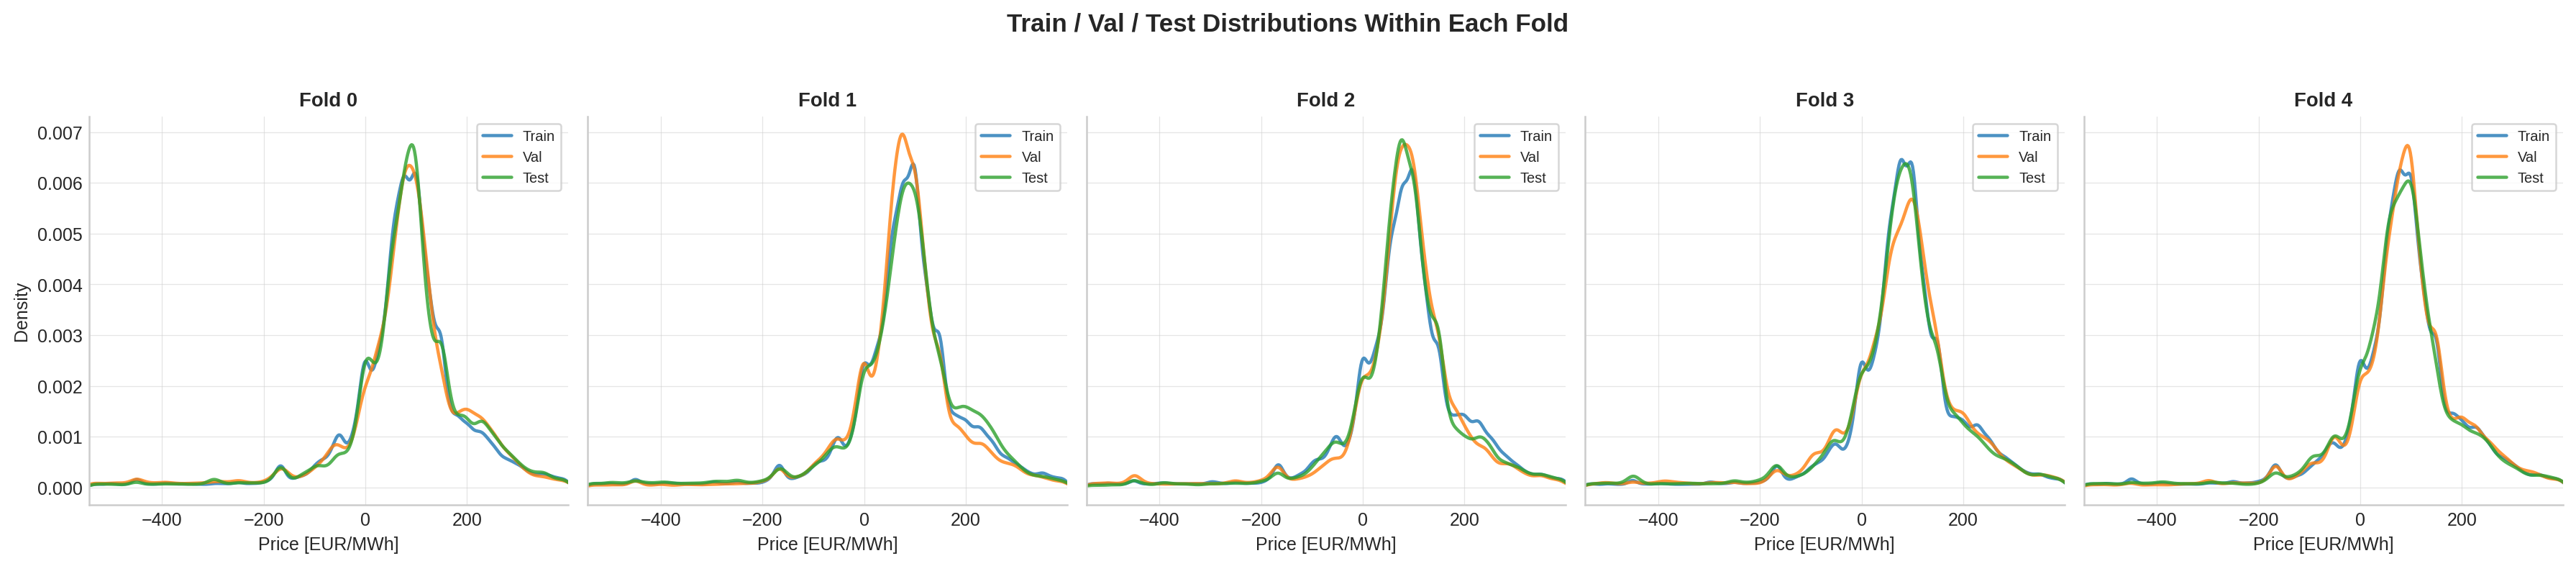
\includegraphics[width=\textwidth]{images/data/difference_between_folds.png}
    \caption{Empirical distribution of imbalance prices compared across the five distinct cross-validation folds.} 
    \label{fig:feature_histograms_between_folds}
\end{figure}

\begin{figure}[h]
    \centering
    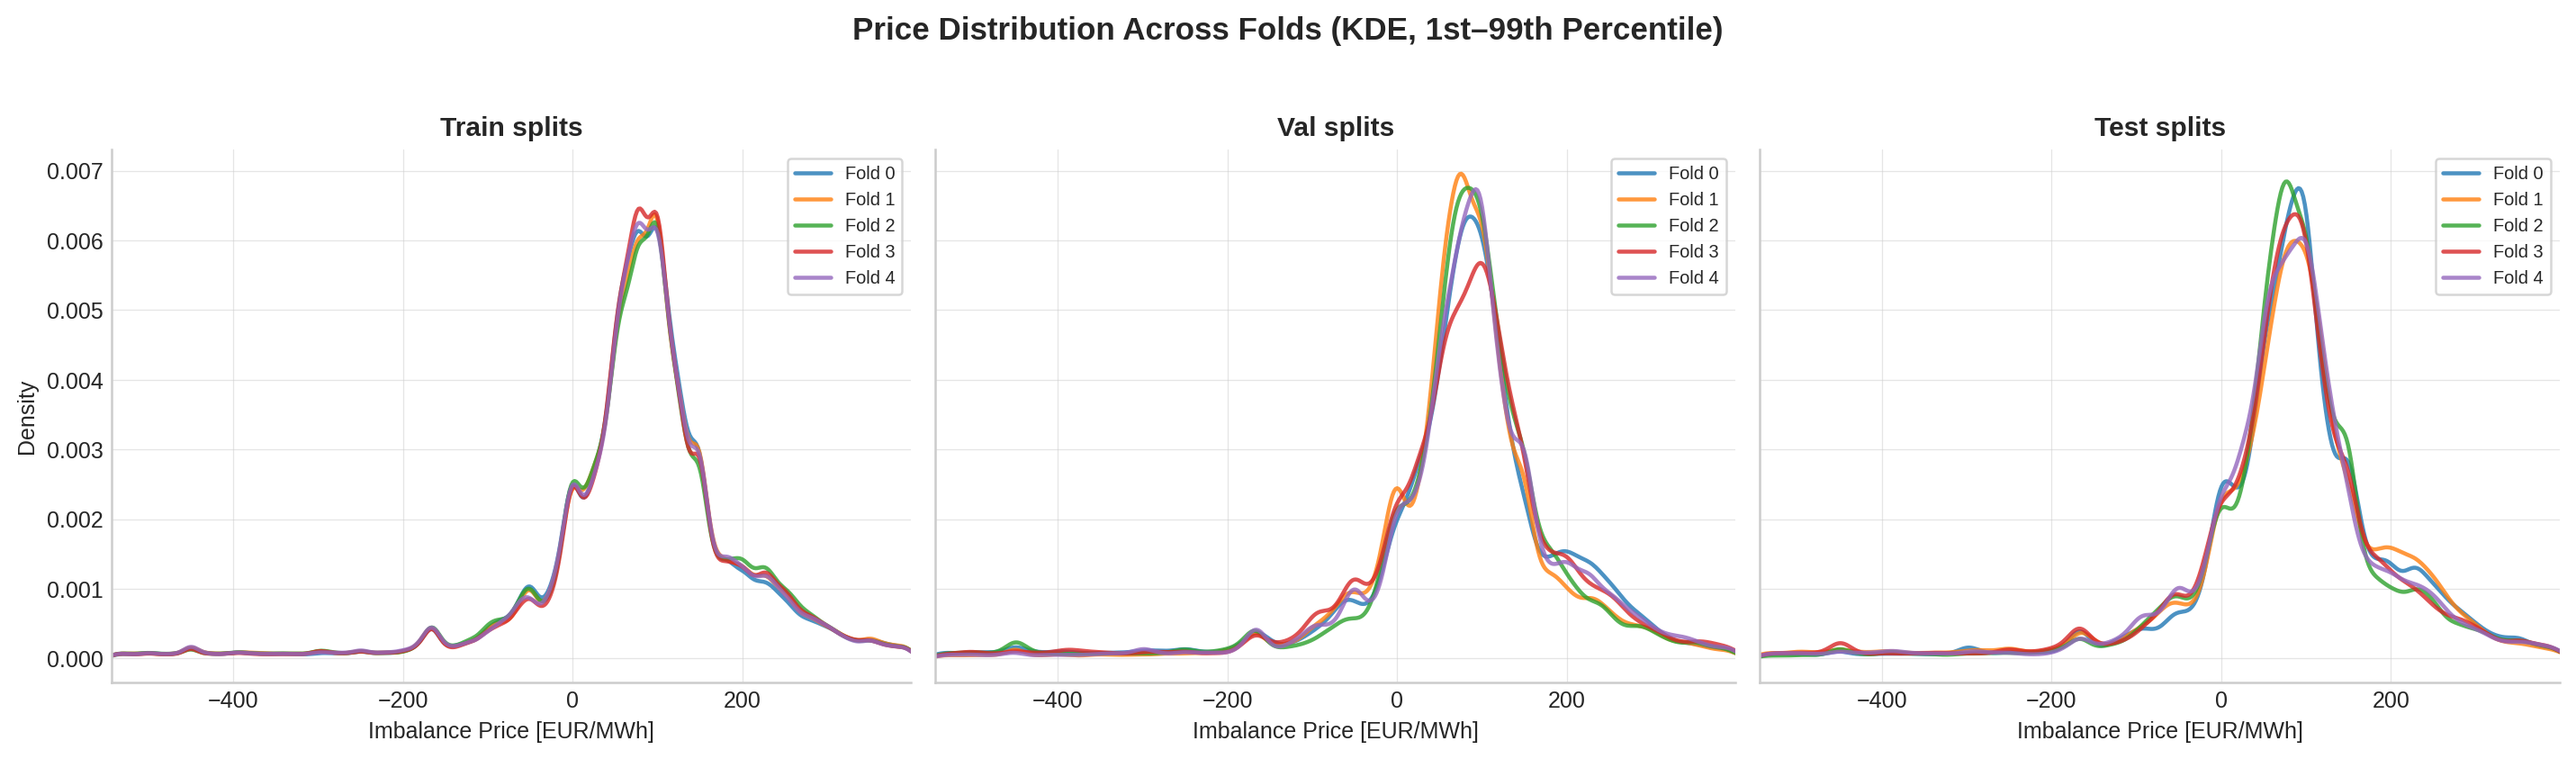
\includegraphics[width=\textwidth]{images/data/difference_inside_fold.png}
    \caption{Empirical distribution of imbalance prices compared across the Training, Validation, and Testing partitions within a representative fold.} 
    \label{fig:feature_histograms_inside_folds}
\end{figure}

As illustrated in Figure \ref{fig:feature_histograms_between_folds}, the empirical distributions of the imbalance prices are highly consistent across all five folds. Furthermore, this consistency holds across the Training, Validation, and Testing sets within the individual folds, as seen in Figure \ref{fig:feature_histograms_inside_folds}. This homogeneity confirms that the $hv$-block cross-validation sampling successfully captured a representative cross-section of the market in all partitions. It provides mathematical validation that this splitting methodology successfully avoids the seasonal biases inherent in chronological splitting.

\subsubsection{The Challenge of Latent Variables}
While the visible imbalance price feature is consistently distributed, the imbalance market is heavily influenced by \textit{latent variables}---factors that drive the price but are not explicitly provided in the agent's observation space (e.g., real-time grid frequency deviations, underlying seasonality, and intermittent renewable generation).

Because the agent cannot directly observe these underlying physical drivers, it must attempt to infer them purely from the movement of the imbalance price. This partial observability introduces an element of \textit{irreducible error} into the learning process. The agent cannot make perfect predictions because it simply lacks the full context of the environment. 

A primary focus of a subsequent chapter in this thesis will be to identify proxies for these latent variables. By engineering new features (such as time-aware encodings and historical price sequences) and systematically adding them to the state space, the objective is to reduce this irreducible error, thereby enabling the agent to learn a more optimal and profitable policy.

\subsubsection{Data usage}
This is maybe in a section after the first evaluation, so this section might need to move.

But it is an interesting question to ask if this model needs this much data, what would be too little data?

